\documentclass[a4paper,british]{article}

\usepackage[utf8]{inputenc}
\usepackage[T1]{fontenc}
\usepackage[british]{babel}

\usepackage[pdfusetitle,colorlinks]{hyperref}
\usepackage[dvipsnames]{xcolor}

\usepackage{lmodern}

\usepackage{bookml/bookml}
\bmlAltFormat{bookmlleeds.pdf}{PDF (serif)}
\bmlAltFormat{bookmlleeds-sans.pdf}{PDF (sans serif)}
\bmlAltFormat{bookmlleeds-sans-large.pdf}{PDF (sans, large)}

\usepackage{geometry}
\ifcsname bmlCrop\endcsname
\usepackage{crop}
\fi

% collapsible titled frame
\usepackage{amssymb}
\usepackage{framed}
\iflatexml
  % if compiling via LaTeXML, emit <DETAILS><SUMMARY>... tags
  \newenvironment{foldedframe}[1][]{%
    \<DETAILS>\<SUMMARY>\textbf{#1}\</SUMMARY>}%
  {\</DETAILS>}
\else
  % if compiling to PDF, emit {titled-frame} using the framed package
  \newenvironment{foldedframe}[1][]{\bgroup\colorlet{TFFrameColor}{SpringGreen}
  \colorlet{TFTitleColor}{black}\begin{titled-frame}{#1}}{\end{titled-frame}\egroup}
\fi

\usepackage{enumitem}

\usepackage{tabularx}
\renewcommand\tabularxcolumn[1]{m{#1}}% for vertical centering text in X column

\usepackage{fancyhdr}
\usepackage{geometry}
\setlength{\parindent}{0pt}
\setlength{\parskip}{0.3em}

\usepackage[all]{xy}
\def\tikzname{Ti\emph{k}Z}

\usepackage{tikz}
\usetikzlibrary{cd}

% for code with syntax highlighting
\usepackage{listings}
\lstset{basicstyle={\small\ttfamily},%
  keywordstyle={\color{blue}\bfseries},%
  keywordstyle=[2]{\color{MidnightBlue}\bfseries},%
  stringstyle={\color{red}},%
  commentstyle={\color{OliveGreen}},%
  frame={single},frameround={tttt},rulecolor={\color{SpringGreen}},%
  upquote=true%
}

\lstdefinelanguage{LaTeX}[LaTeX]{TeX}{%
  moretexcs={chapter,text,RequirePackage,includegraphics,bf}%
}

\lstdefinestyle{latexml}{language=LaTeX,%
  texcsstyle=*{\color{blue}\bfseries},%
  texcsstyle=*[2]{\color{MidnightBlue}\bfseries},%
  moretexcs=[2]{LaTeXML,iflatexml,lxAddClass,lxWithClass,lxBeginTableHead,lxEndTableHead,%
    lxFcn,lxID,lxPunct,lxContextTOC,lxNavbar,lxHeader,lxFooter,ldsHTML,bmlRawHTML,%
    bmlImageEnvironment,bmlDescription,bmlHTMLEnvironment,bmlHTMLInlineEnvironment,bmlDisableMathJax,<,}%
  }

\def\ltxinline{\lstinline[style=latexml,frame=none]}
\def\cmdinline{\lstinline[language=bash,frame=none]}

\title{The Leeds BookML guide}
\author{Vincenzo Mantova}

\date{3\textsuperscript{rd} October 2024}

\begin{document}

\begin{lxFooter}
  Copyright \copyright{} 2021--24 Vincenzo Mantova, University of Leeds.
\end{lxFooter}
\fancyfoot[L]{Copyright \copyright{} 2021--24 Vincenzo Mantova, University of Leeds.}
\fancyfoot[C]{}
\fancyfoot[R]{\thepage}
\pagestyle{fancy}

\maketitle

\begin{abstract}
  A self-contained guide to BookML as used at the University of Leeds: how to convert (virtually any) \LaTeX{} file to zip and SCORM packages with both \HTML{} and PDF versions of all files.
\end{abstract}


\tableofcontents

\section{Installation}
\subsection{Prerequisites}

\begin{foldedframe}[Full list of prerequisites]
  \begin{itemize}
    \item \LaTeXML{} (minimum 0.8.5, recommended 0.8.8 or later)
    \item Any image handling: the Perl module \texttt{Image::Magick}
    \item Support for EPS, PDF images: Ghostscript
    \item BookML images: Ghostscript, \texttt{latexmk}, \texttt{preview.sty}, \texttt{dvisvgm} (minimum 1.6, recommended 2.7 or later)
    \item Automatic PDF, \HTML, and zip creation: GNU Make, \texttt{latexmk}, \texttt{zip}, optionally \texttt{texfot}
  \end{itemize}
\end{foldedframe}

The packages \texttt{latexmk}, \texttt{preview.sty}, \texttt{dvisvgm} and \texttt{texfot} are distributed by MiK\TeX{}, \TeX{} Live, and virtually all Linux distributions.

For the rest of the software, follow the instructions below.

\begin{foldedframe}[macOS (MacPorts)]
  \begin{itemize}
    \item Open the Terminal app.
    \item Run \cmdinline|xcode-select --install| to get the Command Line Developer Tools.
    \item Install MacPorts as per \href{https://www.macports.org/install.php}{its official instructions} \textbf{from point 2} (no need for full Xcode!).
    \item If your \LaTeX{} was installed via Mac\TeX{}, run:
          \begin{lstlisting}
sudo port install LaTeXML +mactex
        \end{lstlisting}
        For the Ghostscript prerequisites, depending on your specific version of Mac\TeX{}, you may need to install the \href{https://tug.org/mactex/morepackages.html}{Ghostscript-Extras package}.

          Otherwise
          \begin{lstlisting}[language=bash]
sudo port install LaTeXML
        \end{lstlisting}

      For the remaining prerequisites (such as \texttt{dvisvgm}), add them as you would add any other \TeX{} Live package (for instance using the \TeX{} Live Utility).
    \item If, \textbf{and only if}, your \LaTeX{} was installed via MacPorts, you can add the optional packages via:
          \begin{lstlisting}[language=bash]
# for automatic PDF, html, zip creation
sudo port install dvisvgm latexmk
# for BookML images (preview.sty)
sudo port install texlive-latex-extra
# for texfot (to reduce latex output during PDF creation)
sudo port install texlive-bin-extra
          \end{lstlisting}
    \item To upgrade:
          \begin{lstlisting}
sudo port selfupdate
sudo port upgrade outdated
        \end{lstlisting}
    \item The remaining packages (e.g. GNU Make) are already available.
  \end{itemize}
\end{foldedframe}

\begin{foldedframe}[macOS (Homebrew) -- PARTLY BROKEN]
  The Homebrew version has intrinsic packaging issues and \textbf{should be avoided}. However, if you really insist:
  \begin{lstlisting}
brew install latexml
    \end{lstlisting}
  Functionality related to images will likely be broken.
\end{foldedframe}

\begin{foldedframe}[Linux Debian-based (Ubuntu, Debian, Mint, etc)]
  Download the package for the \textbf{future} Ubuntu releases at \url{https://launchpad.net/ubuntu/+source/latexml}. At the time of writing, this is \texttt{\href{https://launchpad.net/ubuntu/+archive/primary/+files/latexml_0.8.8-1_all.deb}{latexml\_0.8.8-1\_all.deb}}. Install \texttt{ghostscript}, \texttt{make}, \texttt{latexmk}, \texttt{dvisvgm}, \texttt{preview-latex-style}, \texttt{texlive-extra-utils} (for \texttt{texfot}), \texttt{zip}, according to your needs.
  \begin{lstlisting}
sudo dpkg -i latexml_0.8.8-1_all.deb
sudo apt -f install
sudo apt install ghostscript make latexmk dvisvgm preview-latex-style texlive-extra-utils zip
  \end{lstlisting}
\end{foldedframe}

\begin{foldedframe}[Linux RPM-based (Red Hat, CentOS, AlmaLinux, etc)]
  Not figured out yet!
\end{foldedframe}

\begin{foldedframe}[Linux School PC (presumably only desktop connected via cable)]
  Run the following each time you open a new terminal:
  \begin{lstlisting}
module load latexml
module load texlive
    \end{lstlisting}
  If it does not work, run the following command and try again:
  \begin{lstlisting}
module use /apps/linsw1/modulefiles/7/
    \end{lstlisting}
  Everything else should already be available.
\end{foldedframe}

\begin{foldedframe}[Windows (AppsAnywhere --- easiest, now works offline too)]
  By far the easiest method. It also work in the Windows Virtual Desktop (very slowly!).
  \begin{itemize}
    \item Make sure to have \href{https://it.leeds.ac.uk/it?id=kb_article&sysparm_article=KB0014827}{AppsAnywhere} installed.
    \item Install Ghostscript, ImageMagick, MiK\TeX{}, StrawberryPerl.
    \item Open StrawberryPerl and run:
          \begin{lstlisting}
cpanm --build-args=CC=c++ --notest --verbose Image::Magick
cpanm --notest --verbose LaTeXML
        \end{lstlisting}
  \end{itemize}
  Everything else should then be available. Re-do all of the above to update. You may have to reinstall the apps every one or two months (open the CloudPaging Player to check their status).
\end{foldedframe}

\begin{foldedframe}[Windows (with admin rights)]
  For University laptops: you can gain admin rights by right-clicking an the installer and choosing ``Request Run as Administrator''.
  \begin{itemize}
    \item Install \href{https://strawberryperl.com/}{StrawberryPerl} \texttt{64bit} version.
    \item Install \href{https://imagemagick.org/script/download.php#windows}{ImageMagick} \texttt{x64-dll}. During installation, enable `Install development headers and libraries for C and C++':
    \begin{center}
      % change width on PDF only
      \iflatexml
        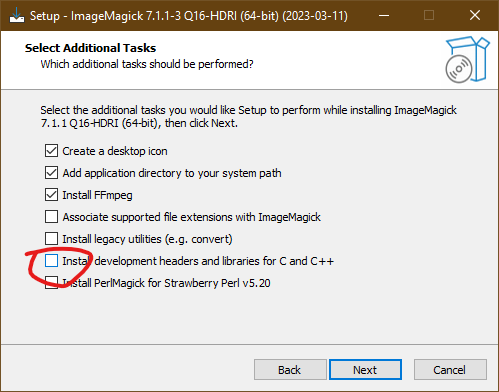
\includegraphics{imagemagick-installer-screenshot.png}
      \else
        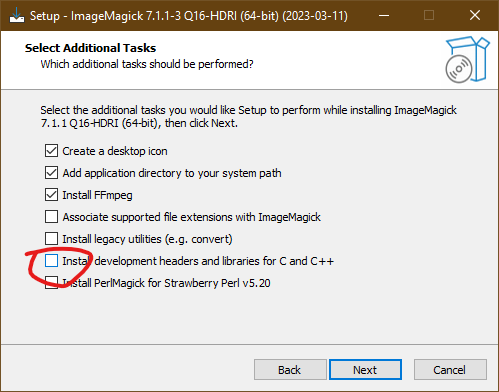
\includegraphics[width=6cm]{imagemagick-installer-screenshot.png}
      \fi
    \end{center}
    Be very careful \textbf{not} to choose 32bit, portable, or static variants.
    \item Install \href{https://www.ghostscript.com/download/gsdnld.html}{Ghostscript} 64bit.
    \item In StrawberryPerl, run
          \begin{lstlisting}
cpanm --build-args=CC=c++ --notest --verbose Image::Magick
cpanm --notest --verbose LaTeXML
    \end{lstlisting}
  \end{itemize}
  Everything else should then be available. Re-do all of the above to update.
\end{foldedframe}

\begin{foldedframe}[Windows (without admin rights)]
  Install the \href{https://scoop.sh/}{Scoop package manager} (no admin required). Then run:
  \begin{lstlisting}
scoop install perl
scoop install imagemagick
scoop install ghostscript
cpanm --build-args=CC=c++ --notest --verbose Image::Magick
cpanm --notest --verbose LaTeXML
    \end{lstlisting}
  Everything else should then be available. Use \cmdinline|scoop update --all| to update.
\end{foldedframe}

\begin{foldedframe}[Docker/Podman/etc]
  You can also run BookML using Docker. The default image will compile automatically all the content of the \texttt{/source} folder. For instance:
  \begin{lstlisting}
docker run --rm -i -t -v.:/source ghcr.io/vlmantova/bookml
  \end{lstlisting}
  Please note that the Docker image includes a full copy of TeX Live 2021.
\end{foldedframe}

\subsection{BookML}

Unzip the \texttt{\href{https://github.com/vlmantova/bookml/releases/latest/download/template.zip}{template.zip} }file from the \href{https://github.com/vlmantova/bookml/releases/latest}{latest BookML release}. Open a terminal in the directory containing \texttt{Makefile}, \texttt{template.tex}, and run
\begin{lstlisting}
make detect
\end{lstlisting}
\dots or \cmdinline|gmake detect| on Windows.

\begin{foldedframe}[How do I run commands in the terminal?]
  You simply type them and press \texttt{<ENTER>}. To open the terminal in a specific folder:

  \begin{foldedframe}[Windows]
    Install the \href{https://github.com/microsoft/terminal?tab=readme-ov-file#via-windows-package-manager-cli-aka-winget}{Windows Terminal}. The easiest way is from the \href{https://apps.microsoft.com/store/detail/windows-terminal/9N0DX20HK701}{Microsoft Store}. If the Store is blocked, you can use
    \begin{lstlisting}
winget install --id Microsoft.WindowsTerminal -e
    \end{lstlisting}

    You will then be able to right-click on the folder and select ``Open in Windows Terminal''.
  \end{foldedframe}
  \begin{foldedframe}[macOS]
    Right-click on a folder and select ``New Terminal at Folder''.
  \end{foldedframe}
  \begin{foldedframe}[Linux]
    Many file browsers have an option ``Open in Terminal'' when you right-click on a folder.
  \end{foldedframe}
\end{foldedframe}

Use \cmdinline|gmake detect| on Windows. You should get something like the following:

\begin{tabular}[h]{>{\color{MidnightBlue}\tt}r@{\texttt{\ }}>{\tt}l}
  Main files:    & \color{OliveGreen} template.tex                               \\
  BookML:        & \color{OliveGreen} v0.4.3 OK                                               \\
  GNU Make:      & \color{OliveGreen} 4.4.1 OK                                                \\
  TeX:           & \color{OliveGreen} MiKTeX 24.1 OK                            \\
  perl:          & \textcolor{OliveGreen}{v5.38.0 OK} (optional)                            \\
  LaTeXML:       & \color{OliveGreen} 0.8.7 OK                                              \\
  Image::Magick: & \textcolor{OliveGreen}{7.1.1 OK} (required for any image handling)      \\
  Ghostscript:   & \textcolor{OliveGreen}{10.02.1 OK} (required for EPS, PDF, BookML images) \\
  dvisvgm:       & \textcolor{OliveGreen}{3.1.1 OK} (required for SVG, BookML images)      \\
  dvisvgm/libgs: & \textcolor{OliveGreen}{9.25 OK} (required for SVG, BookML images)      \\
  latexmk:       & \color{OliveGreen} 4.82a OK                                             \\
  texfot:        & \textcolor{OliveGreen}{1.48 OK} (optional)                               \\
  preview.sty:   & \textcolor{OliveGreen}{13.3 OK} (required for BookML images)             \\
  zip:           & \color{OliveGreen} 3.1b OK
\end{tabular}

Anything missing will show a red \textcolor{red}{\tt NOT FOUND}. If the version is too old, there will be a red or a yellow prompt to upgrade.

\textbf{First try?} Run \cmdinline|make| (or \cmdinline|gmake| on Windows). After a bit, you will find a folder \texttt{template} and two zip files \texttt{template.zip}, \texttt{SCORM.template.zip}. Please open \texttt{template/index.html} and verify that it looks as you would expect. The zip files are set up for upload on Minerva.

\textbf{To update BookML}, simply replace the \texttt{bookml} folder with the content of a newly downloaded \href{https://github.com/vlmantova/bookml/releases/latest/download/bookml.zip}{\texttt{bookml.zip}}.

\section{Converting your files}

\subsection{How to convert}
Once your are satisfied that the template is working, drop your own files next to \texttt{template.tex}: each file containing \ltxinline|\documentclass| will be treated the same as \texttt{template.tex}, and will be compiled to PDFs, SCORM and zip packages. Run \cmdinline|make detect| again, and check that `Main files' contains such new files.

There is now a reasonable chance that your files are already working (unless you are using \tikzname, which needs some care), but before your first try, you should truncate your files with an early \ltxinline|\end{document}|, as compilation times can be long and most errors will originate in the preamble anyway.

To compile, do the following:
\begin{itemize}
  \item Run
        \begin{lstlisting}
make
        \end{lstlisting}
        On Windows, it is \cmdinline|gmake| rather than \cmdinline|make|.

        After a bit, you will have files named like \texttt{lecturenotes.zip}, \texttt{SCORM.lecturenotes.zip}. The former works with `Upload Zip package'; the latter with `Create SCORM package'.

        To generate one particular package, for instance the one for the file \texttt{lecturenotes.tex}, run
        \begin{lstlisting}
make lecturenotes.zip
        \end{lstlisting}
        or, if you are using SCORM packages,
        \begin{lstlisting}
make SCORM.lecturenotes.zip
        \end{lstlisting}
  \item When you change a file and want to regenerate the zip files, just run \cmdinline|make| again. Only the files that need updating will be recompiled.
  \item You may occasionally get errors like
        \begin{lstlisting}
No rule to make target 'bookml-short-guide.toc', needed by 'auxdir/bookml-short-guide.pdf'.
        \end{lstlisting}
        If that happens, run \cmdinline|make| a second time. If the error is still there, run \cmdinline|make clean-aux|, or delete the \texttt{auxdir} folder, to reset BookML.
\end{itemize}

\begin{foldedframe}[What is \texttt{make} doing? Step-by-step look under the hood]
  Each time you call \texttt{make}, it does the following.
  \begin{enumerate}[start=0]
    \item Read the file \texttt{Makefile} in the folder you are in. That file will import instructions from the \texttt{bookml} folder about what to do next.

    \item \label{find-main} Check all \texttt{.tex} files in the folder and find the ones containing \ltxinline|\documentclass|.

    {\small In \texttt{example.zip}, it finds \texttt{main.tex} and \texttt{secondfile.tex}.}

    \item \label{targets} Arrange to generate two `targets', a zip package and a SCORM package, for every such file in step~\ref{find-main}.

    {\small In the example, the targets are \texttt{main.zip}, \texttt{SCORM.main.zip}, \texttt{secondfile.zip}, \texttt{SCORM.secondfile.zip}.}

    \item \label{prereqs} Check if the targets of step~\ref{targets} exist, and if so, if any of their `prerequisites' are newer, in which case the targets must be updated. The prerequisites themselves are checked recursively to see if they also need to be updated. The prerequisite chain looks like `\texttt{zip => html => xml => pdf => tex}'.

    {\small In the example, on your first try, Make will follow the following prerequisite chain: \texttt{main.zip => main/index.html => main.xml => main.pdf => main.tex}. It will then build the prerequisites backwards until all is in place to create \texttt{main.zip}. Likewise for the other targets.}

    \item \label{pdfs} Build the PDF of each \LaTeX{} file found in step~\ref{find-main}, using \texttt{latexmk} to run \texttt{pdflatex}, \texttt{makeindex}, \texttt{bibtex} and similar as many times as necessary; record which files are \ltxinline|\input|'d and mark them as prerequisites for step~\ref{prereqs}.

    {\small In the example, it builds \texttt{main.pdf}, \texttt{secondfile.pdf}, and marks \texttt{chapter1.tex} as prerequisite of \texttt{main.pdf}. Any update to \texttt{chapter1.tex} will cause \texttt{main.pdf} to be updated next time you call \texttt{make}.}

    \item Call \LaTeXML{} to build an \XML{} file from each file in step~\ref{find-main}.

    {\small In the example, \texttt{main.xml}, \texttt{secondfile.xml}.}

    \item Try to build or update the alternative formats requested using \ltxinline|\bmlAltFormat|. For now, BookML only knows how to build PDF files from \LaTeX{} files that have the same name; if you need other formats, you need to build them yourself, or add the relevant instructions (called `recipes') in the \texttt{Makefile}.

    {\small In the example, \texttt{main-sans.pdf} and \texttt{main-sans-large.pdf} are the alternative formats requested in the preamble of \texttt{main.tex}, on top of \texttt{main.pdf} which has been built already. Since the example contains \texttt{main-sans.tex}, \texttt{main-sans-large.tex}, BookML will know what to do, and generate the alternative PDFs by repeating step~\ref{pdfs}.}

    \item Convert the \XML{} files to \HTML{}, using \texttt{latexmlpost}.

    {\small Thus generate the folders \texttt{main}, \texttt{secondfile}, each containing an \texttt{index.html}.}

    \item Zip the folder and pack the SCORM package (the latter requiring a couple more steps I will not explain), using \texttt{zip}

    {\small At last, you will get \texttt{main.zip}, \texttt{SCORM.main.zip}, \texttt{secondfile.zip}, \texttt{SCORM.secondfile.zip}.}
  \end{enumerate}
\end{foldedframe}

\subsection{Necessary adjustments}
Consult \texttt{template.tex} for the minimal requirements in the preamble (e.g.\ you \textbf{must} provide a \ltxinline|\title| command). You should create copies of \texttt{template-sans.tex}, \texttt{template-sans-large.tex} for each of your main files, at least as a baseline. Alternative versions can be customized and removed, as explained in the next subsection. We recommend offering some alternative versions as good practice.

You should also follow the key requirements below.
\begin{itemize}
  \item Use the \ltxinline|babel| package to set the document language (crucial for screen readers to work correctly). For instance:
        \begin{lstlisting}[style=latexml]
\usepackage[british]{babel}
  \end{lstlisting}
  \item Set the document metadata in the preamble (essential for proper navigation links, web page titles, SCORM package metadata, and so on).
        \begin{lstlisting}[style=latexml]
\title{LaTeXML + BookML guide}
\author{Vincenzo Mantova}
    \end{lstlisting}
  \item Ensure all \TeX{} style formatting commands (\ltxinline|\Large|, \ltxinline|\bf|, \dots) are enclosed between braces, and use \LaTeX{} alternatives such as \ltxinline|\textbf{}| when possible. If you see the wrong font in the \HTML{} output, it is likely caused by \TeX{}-style font switches that haven't gone well.
        \begin{lstlisting}[style=latexml]
{\bf some bold text}    % DO
\bf some bold text      % DON'T
\textbf{some bold text} % BEST
    \end{lstlisting}
  \item Using \tikzname{} or \Xy-pic and an old version of \LaTeXML{} (before 0.8.7)? Follow the instruction below right away. Without it, \LaTeXML{} will take several minutes longer (regardless of the size of the file) and often produce broken images. Since version 0.8.7, \LaTeXML{} has become more capable, and 0.8.8 can produce excellent \tikzname{} pictures as well as \texttt{tikzcd} diagrams.
\end{itemize}

\subsection{Alternative formats}
To create an alternative PDF meant to be included in the same SCORM or zip package (such as a large print PDF), for instance for the \texttt{lecturenotes.zip} package, add the following to the preamble of \texttt{lecturenotes.tex}:
\begin{lstlisting}[style=latexml]
  \usepackage{bookml/bookml} % if not already in your preamble
  \bmlAltFormat{lecturenotes.LARGE.pdf}{PDF (large print)}
\end{lstlisting}
and create a corresponding \texttt{lecturenotes.LARGE.tex} that
\begin{itemize}
  \item does \textbf{NOT} contain \ltxinline|\documentclass| (or it will be compiled into its own SCORM and zip packages);
  \item configures e.g.\ different fonts and margins, then call \ltxinline|\input{lecturenotes.tex}|.
\end{itemize}
BookML will automatically compile and include \texttt{lecturenotes.LARGE.pdf} in your final outputs.

Consult \texttt{template.tex}, \texttt{template-sans.tex}, \texttt{template-sans-large.tex} for some simple techniques to achieve this.

If you instead want \textbf{distinct} SCORM and zip packages, for instance compile a problem sheet both with and without solutions, explore \href{https://github.com/vlmantova/bookml/releases/latest/download/template.zip}{\texttt{example.zip}} to see some possibilities.

\subsection{Other adjustments}
Once you have language and metadata in place, follow the advice below to improve the chances your file will compile correctly, \textbf{especially if you use \tikzname{} or \Xy}.

\begin{foldedframe}[Many or complex \tikzname{} pictures]
  BookML has a facility to generate the images via \LaTeX{}, bypassing \LaTeXML{}'s internal SVG generator, which sometimes fails to create good \tikzname{} pictures.

  If you are running \LaTeXML{} 0.8.8, most \tikzname{} figures should render reasonably well. If one particular figure causes issues, wrap it in \ltxinline|\begin{bmlimage}| and \ltxinline|\end{bmlimage}|.

  If the issues affect several images, you can run \emph{all} \tikzname{} figures automatically via BookML by doing the following. First, ensure that \textbf{all of the} \tikzname{} code is either in the preamble or between \ltxinline|\begin{tikzpicture}| and \ltxinline|\end{tikzpicture}| (this will speed up compilation). Then add the following to the preamble, after the bookml package:
  \begin{lstlisting}[style=latexml]
\bmlImageEnvironment{tikzpicture}
\bmlImageEnvironment{tikzcd} % if using tikzcd
\iflatexml
\else
\usepackage{tikz}
% ... ALL of the TikZ-related preamble code here
\fi
% No TikZ commands after this point!
\end{lstlisting}
  See \autoref{fig:tikz-example}, \autoref{fig:tikzcd-example}.
\end{foldedframe}

\begin{foldedframe}[Other figures, e.g.\ \Xy-matrices or \texttt{animate}]
  Most packages producing pictures are not supported by \LaTeXML{}, but you can get around it exactly like with \tikzname{}:
  \begin{enumerate}
    \item wrap the preamble commands within \ltxinline|\iflatexml\else ... \fi|;
    \item if the pictures are their own environments, use \ltxinline|\bmlImageEnvironment| as for \tikzname{}; see for instance \autoref{fig:tikzcd-example};
    \item if the pictures are not environments, such as \ltxinline|\xymatrix|, wrap them between \ltxinline|\begin{bmlimage}| and \ltxinline|\end{bmlimage}|: see \autoref{fig:xymatrix-example}.
  \end{enumerate}
  You can read more details and see examples in \href{https://vlmantova.github.io/bookml}{BookML manual}.
  \par
  \LaTeXML{} 0.8.7 has experimental native support for \Xy-matrices, but it is still not very good.
\end{foldedframe}
\begin{foldedframe}[Alternative text for images (essential for screen readers)]
For \ltxinline|\includegraphics| and \LaTeXML{} 0.8.7, just add the option \ltxinline|alt={description of the image}|, as in
\begin{lstlisting}[style=latexml]
\includegraphics[alt={Computation of ...}]{figure1}
\end{lstlisting}

For older versions, and other images such as \tikzname{} pictures, add \ltxinline|\bmlDescription{text}| right after the image (do not leave an empty line between the image and the text). This will populate the \texttt{alt} attribute (or equivalent) and will be read by screen readers in place of the image.

Please keep in mind that sighted users may also benefit from the alternative text. If that is the case, consider using \ltxinline|\begin{figure}| and \ltxinline|\caption{}|, and possibly add a reference in the caption to more explanations (e.g.\ the definition, a proof, etc.).
\end{foldedframe}
\begin{foldedframe}[Table headers (important for screen readers)]
  You may need to explicitly mark some table rows as headers. This can be done with some appropriate commands provided by \LaTeXML{}. See \autoref{fig:table} for an example.
\end{foldedframe}
\begin{foldedframe}[Split into multiple pages]
  Add \cmdinline|SPLITAT=chapter| to \texttt{Makefile} to split the output in various ways (you can use part, chapter, section\dots{}). You \textbf{must} split long documents, or MathJax will take ages to render your formulas.

  You can also specify different splitting strategies for different files: add lines like the following
  \begin{lstlisting}
lecturenotes.zip: SPLITAT=section
problemsheet1.zip: SPLITAT=
\end{lstlisting}
  to the end of \texttt{Makefile}. The above will split \texttt{lecturenotes.tex} into a page per section, and will not split \texttt{problemsheet1.tex}. By default, files will be split by chapter.
\end{foldedframe}
\begin{foldedframe}[Disable the bookdown style]
  If you do not like the bookdown style and prefer a more plain page, like the old \texttt{latexmlleeds}, use
  \begin{lstlisting}[style=latexml]
\usepackage[style=plain]{bookml/bookml}
  \end{lstlisting}
  You may wish to disable the additional table of contents, for instance add
  \begin{lstlisting}
lecturenotes.zip: LATEXMLPOSTEXTRAFLAGS=--navigationtoc=none
  \end{lstlisting}
  at the end of \texttt{Makefile}. See `Split into multiple pages' for more details.
\end{foldedframe}
\begin{foldedframe}[Navigation sidebar]
  This is already included in the bookdown style. If you disable it, but still want the sidebar, add
  \begin{lstlisting}
lecturenotes.zip: LATEXMLPOSTEXTRAFLAGS=--css=LaTeXML-navbar-left.css
  \end{lstlisting}
  to the end of \texttt{Makefile}.
\end{foldedframe}
\begin{foldedframe}[Customise \CSS{} (fonts, color)]
  Create the \texttt{bmluser} folder and add \CSS{} files to it.
\end{foldedframe}
\begin{foldedframe}[Embed videos]
  You can use \ltxinline|\bmlRawHTML{html}| to write arbitrary \HTML{}, in particular output the embedding code for Stream, Mediasite, YouTube, or any other platform. Unfortunately, Microsoft Stream Classic is being phased out and may be broken in some browsers.

  See \autoref{fig:embed-stream} below for some reusable code that will also make the video adapt to the size of the page.
\end{foldedframe}
\begin{foldedframe}[Unsupported packages or classes]
  \LaTeXML{} supports only so many packages (\href{https://dlmf.nist.gov/LaTeXML/manual/included.bindings/}{full list}). If your package is not supported, or is not supported well, see \autoref{sub:unsupported-packages}.
\end{foldedframe}
\begin{foldedframe}[Resize BookML images (deprecated)]
  To change the size of the BookML images, use
  \begin{lstlisting}[style=latexml]
\usepackage[imagescale=2.5]{bookml/bookml}
  \end{lstlisting}
  Please note that images are now resized so that the text within the images has roughly the same sizes as the surrounding page. The option \ltxinline|imagescale| will eventually disappear.

  For images converted by \LaTeXML{}, starting with 0.8.7, you can try the following experimental and undocumented options:
  \begin{lstlisting}[style=latexml]
\usepackage[dpi=192,magnify=2,upsample=3,zoomout=2]{latexml}
  \end{lstlisting}
  although you are \textbf{strongly recommended} to convert EPS and PDF images by yourself separately to SVG, using for instance \texttt{dvisvgm}, to get substantially better quality.
\end{foldedframe}
\begin{foldedframe}[Foldable environments]
  If you want to hide a proof, a solution, or some additional details, you can use the following:

  \begin{lstlisting}[style=latexml]
\<DETAILS>
  \<SUMMARY>\textbf{Solution.}\</SUMMARY>
  ...details of the solutions...
\</DETAILS>
    \end{lstlisting}
  More generally, you can add arbitrary \HTML{} tags by starting them with \ltxinline|\<|, and using the \XML{} syntax (for instance, attributes must have values between quotes, self-closing tags must end with \ltxinline|/>|).

  If you like the styling used here, just drop the \href{bmluser/bookmlleeds-details.css}{bookmlleeds-details.css} file into the \texttt{bmluser} folder.
\end{foldedframe}
\begin{foldedframe}[Customize header and footer (e.g.\ for copyright notice)]
  Use the environments \ltxinline|lxHeader|, \ltxinline|lxFooter|.
  \begin{lstlisting}[style=latexml]
\begin{lxFooter}
  Copyright \copyright{} 2021 Vincenzo Mantova, University of Leeds.
\end{lxFooter}
    \end{lstlisting}
  The header is omitted in the bookdown (GitBook) style.
\end{foldedframe}
\begin{foldedframe}[Disable MathJax for an equation]
  Add \ltxinline|\bmlDisableMathJax| within the equation. Please review the output in Firefox, Safari, and Chrome/Edge (from versions 109).
\end{foldedframe}
\begin{foldedframe}[Other options]
  Visit the \href{https://vlmantova.github.io/bookml}{BookML documentation}, the \href{https://dlmf.nist.gov/LaTeXML/docs.html}{\LaTeXML{} documentation}, or run \cmdinline|latexml --help|, \cmdinline|latexmlpost --help|, \cmdinline|latexmlc --help|.
\end{foldedframe}

\subsection{Unsupported packages or classes}
\label{sub:unsupported-packages}
If \LaTeXML{} does not recognise a particular package or class, it is sometimes easy to make it work, but it can also be near impossible.
\begin{itemize}
  \item If you use your own custom-made package or class to keep your favourite packages and options (so essentially a fancy preamble): change its extension to \texttt{.tex} and use \ltxinline|\input| instead of \ltxinline|\usepackage|.
  \item If the package is producing images: use the same strategy as for \tikzname{}, and remember to provide alternative text.
  \item If \LaTeXML{} supports a similar package: replace it (for instance, use \texttt{actuarialangle} instead of \texttt{lifecon}).
  \item If the package is PDF-specific: use \ltxinline|\iflatexml| and \ltxinline|\newcommand| in the preamble to define macros that do something equivalent, or nothing at all, in \HTML{}. Useful, for instance, for references including page numbers, or setting headers and footers.
  \item If the class is not supported, tell \LaTeXML{} to use a different class:
        \begin{lstlisting}[style=latexml]
% just like \usepackage, but before \documentclass
\RequirePackage{bookml/bookml}
\iflatexml
\documentclass[12pt]{book}
\else
\documentclass[12pt]{memoir}
\fi
    \end{lstlisting}
        Make sure you pass your class options are consistent, for instance use the same font size.
  \item If none of the above works, copy the missing macros directly from the package (or class) and add them to your preamble (usually within \ltxinline|\makeatletter| and \ltxinline|\makeatother|). It may work for simple packages, or packages partially supported by \LaTeXML{}.
  \item Generalising the last idea, you can tell \LaTeXML{} to read the entire package or class as if you were using \ltxinline|\input|. To do this, create a file named \texttt{package.sty.ltxml} in the same folder as the \texttt{.tex} file (replace \texttt{package} with the actual package name, and \texttt{sty} with \texttt{cls} if dealing with a class):
        \begin{lstlisting}[language=Perl]
use LaTeXML::Package;
InputDefinitions('package', type => 'sty', noltxml => 1);
1;
  \end{lstlisting}
        This will instruct \LaTeXML{} to read the content of \texttt{package.sty}. This may work wonderfully, or crash miserably.
\end{itemize}

\clearpage
\subsection{Examples}

\begin{figure}[hb]
  \begin{center}
    \begin{bmlimage}
      \begin{tikzpicture}
        \draw (0.5,0.5) node {$2$};
        \draw (1.5,0.5) node {$+$};
        \draw (3,0.5) node {$3$};
        \draw (4.5,0.5) node {$=$};
        \draw (7,0.5) node {$5$};
        \draw (0,0) node [below] {$0$} -- (1,0) node [below] {$1$};
        \draw (1.5,0) node {$+$};
        \draw (2,0) node [below] {$0$} -- (3,0) node [below] {$1$} -- (4,0) node [below] {$2$};
        \draw (4.5,0) node {$=$};
        \draw (5,0) node [below] {$0$} -- (6,0) node [below] {$1$};
        \draw [dashed] (6,0) -- (7,0);
        \draw (7,0) node [below] {$2$} -- (8,0) node [below] {$3$} -- (9,0) node [below] {$4$};
        \foreach \x in {0,1,2,3,4,5,6,7,8,9} {
            \fill (\x,0) circle (0.05);
          }
      \end{tikzpicture}
    \end{bmlimage}
    \bmlDescription{To compute 2+3, add a copy of the well ordered set 3 after the well ordered set 2, and note that the result is isomorphic to the well ordered set 5.}
  \end{center}
  \begin{center}
    \begin{tikzpicture}
      \draw (0.5,0.5) node {$2$};
      \draw (1.5,0.5) node {$+$};
      \draw (3,0.5) node {$3$};
      \draw (4.5,0.5) node {$=$};
      \draw (7,0.5) node {$5$};
      \draw (0,0) node [below] {$0$} -- (1,0) node [below] {$1$};
      \draw (1.5,0) node {$+$};
      \draw (2,0) node [below] {$0$} -- (3,0) node [below] {$1$} -- (4,0) node [below] {$2$};
      \draw (4.5,0) node {$=$};
      \draw (5,0) node [below] {$0$} -- (6,0) node [below] {$1$};
      \draw [dashed] (6,0) -- (7,0);
      \draw (7,0) node [below] {$2$} -- (8,0) node [below] {$3$} -- (9,0) node [below] {$4$};
      \foreach \x in {0,1,2,3,4,5,6,7,8,9} {
          \fill (\x,0) circle (0.05);
        }
    \end{tikzpicture}
    \bmlDescription{To compute 2+3, add a copy of the well ordered set 3 after the well ordered set 2, and note that the result is isomorphic to the well ordered set 5.}
  \end{center}
  \caption{Ordinal sum of $2$ and $3$ generated in two ways: first via `bmlimage', then directly by \LaTeXML{}. The latter uses MathJax for the embedded formulas, resulting in improved accessibility but minor alignment issues.}
  \label{fig:tikz-example}
\end{figure}

\begin{figure}[hb]
  \begin{center}
    \begin{bmlimage}
      \begin{tikzcd}
        A \arrow[rd] \arrow[r, "\phi"] & B \\
        & C
      \end{tikzcd}
    \end{bmlimage}
    \bmlDescription{A, B, C drawn in a triangle with C under B, an arrow labelled phi from A to B and an arrow from A to C}
  \end{center}
  \begin{center}
    \begin{tikzcd}
      A \arrow[rd] \arrow[r, "\phi"] & B \\
      & C
    \end{tikzcd}
    \bmlDescription{A, B, C drawn in a triangle with C under B, an arrow labelled phi from A to B and an arrow from A to C}
  \end{center}
  \caption{Example of tikzcd diagram, again generated in two ways via `bmlimage' and directly by \LaTeXML{}.}
  \label{fig:tikzcd-example}
\end{figure}

\begin{figure}[hb]
  \begin{lstlisting}[style=latexml]
\begin{bmlimage}
  \[ \xymatrix{
        A \ar[rd] \ar^\phi[r] & B \\
                              & C } \]
\end{bmlimage}
\bmlDescription{A, B, C drawn in a triangle with C under B,
  an arrow labelled phi from A to B and an arrow from A to C}
  \end{lstlisting}
  \begin{center}
    \[ \begin{bmlimage} \xymatrix{
          A \ar[rd] \ar^\phi[r] & B \\
      & C } \end{bmlimage} \]
    \bmlDescription{A, B, C drawn in a triangle with C under B, an arrow labelled phi from A to B and an arrow from A to C}
  \end{center}
  \caption{Example of \Xy-matrix diagram processed using \texttt{bmlimage}.}
  \label{fig:xymatrix-example}
\end{figure}
\begin{figure}
  \[ \xymatrix{
      A \ar[rd] \ar^\phi[r] & B \\
      & C } \]
  \caption{Unsatisfying example of \Xy-matrix generated directly by \LaTeXML{}.}
\end{figure}

\begin{figure}[hb]
  \begin{lstlisting}[style=latexml]
% preamble
\newcommand{\includestream}[2]{
  \bmlRawHTML{<div style="max-width: 1920px; width: 100\%">
    <div style="position: relative; padding-bottom: 56.25\%; height: 0; overflow: hidden;">
      <iframe
        src="https://web.microsoftstream.com/embed/video/#1?autoplay=false\&amp;showinfo=true"
        title="#2" style="border:none; position: absolute; top: 0; left: 0;
          right: 0; bottom: 0; height: 100\%; max-width: 100\%;"
        allow="picture-in-picture" allowfullscreen="" width="1920" height="1080">
      </iframe>
    </div></div>}
    Watch \href{https://web.microsoftstream.com/video/#1}{#2}
  }
% document
\includestream{ba6b8866-df29-4dea-a47e-13decc5cd409}{Mock recording for Models and Sets}
  \end{lstlisting}
  \begin{quote}
    \newcommand{\includestream}[2]{
      \bmlRawHTML{<div style="max-width: 1920px; width: 100\%">
        <div style="position: relative; padding-bottom: 56.25\%; height: 0; overflow: hidden;">
        <iframe
        src="https://web.microsoftstream.com/embed/video/#1?autoplay=false\&amp;showinfo=true"
        title="#2" style="border:none; position: absolute; top: 0; left: 0;
        right: 0; bottom: 0; height: 100\%; max-width: 100\%;"
        allow="picture-in-picture" allowfullscreen="" width="1920" height="1080">
        </iframe>
        </div></div>}
      Watch \href{https://web.microsoftstream.com/video/#1}{#2}
    }
    % document
    \includestream{ba6b8866-df29-4dea-a47e-13decc5cd409}{Mock recording for Models and Sets}
  \end{quote}
  \label{fig:embed-stream}
  \caption{How to embed a video. Note that the \LaTeX{} special characters are preceeded by a backslash or the output may be invalid.}
\end{figure}

\begin{figure}[hb]
  \begin{lstlisting}[style=latexml]
\begin{tabularx}{\textwidth}{c|X||c}
  \lxBeginTableHead{} Header 1 & Header 2 & Header 3 \\
  \hline \lxEndTableHead{}
  Content & Content & Content \\
  More content & content & content \\
  \hline
\end{tabularx}
\caption{A table}
  \end{lstlisting}
  \begin{tabularx}{\textwidth}{c|X||c}
    \lxBeginTableHead{} Header 1 & Header 2 & Header 3 \\
    \hline \lxEndTableHead{}
    Content                      & Content  & Content  \\
    More content                 & content  & content  \\
    \hline
  \end{tabularx}
  \caption{Mark a table row as header. Read the content of \href{https://github.com/brucemiller/LaTeXML/blob/master/lib/LaTeXML/texmf/latexml.sty}{\texttt{latexml.sty}} for more table-related commands.}
  \label{fig:table}
\end{figure}

\subsection{The \texttt{latexml.sty} package (advanced)}
The \ltxinline|bookml| package automatically loads the \texttt{latexml.sty} package (and it includes its own copy if \texttt{latexml.sty} is not in your \LaTeX{} installation). \texttt{latexml.sty} offers a variety of commands which may be useful. Just open \href{https://github.com/brucemiller/LaTeXML/blob/master/lib/LaTeXML/texmf/latexml.sty}{\texttt{latexml.sty}} (it is very short) to see all the commands, a bit of documentation in the comments, and the occasional example. The \href{https://github.com/brucemiller/LaTeXML/tree/master/doc/manual}{source} of the \LaTeXML{} documentation contains many examples too. Below are some relevant ones.
\begin{itemize}
  \item \ltxinline|\lxAddClass{class}| and \ltxinline|\lxWithClass{class}{content}| to add \CSS{} classes to the output;
  \item \ltxinline|\lxBeginTableHead|, \ltxinline|\lxEndTableHead| and variations to mark table headers and footers (read the \texttt{latexml.sty} source for how to use them);
  \item \ltxinline|\lxContextTOC|, \ltxinline|\lxNavbar{arg}|, \ltxinline|\lxHeader{arg}|, \ltxinline|\lxFooter{arg}| to customise the \HTML{} pages;
  \item \ltxinline|\lxFcn{code}|, \ltxinline|\lxID{code}|, \ltxinline|\lxPunct{code}| to help \LaTeXML{} understand the meaning of mathematical symbols (for instance, read $f(a+b)$ as `$f$ applied to $a+b$' as opposed to `$f$ multiplied by $a+b$'); the wrong interpretation may affect screen readers, so it will need to be addressed, but for now this is too hard to deal with.
\end{itemize}

\section{Uploading to Minerva}
\subsection{SCORM packages}
\begin{enumerate}
  \item On the front page of your module, under `Module content', click the $\oplus$ button where you want to insert your item.
  \item Choose `$\oplus$ Create'.
  \item Choose `SCORM package'.
  \item Choose `Upload SCORM package' and select your \texttt{SCORM.<...>.zip} file.
  \item Disable `Grade SCORM' and click 'Save'.
\end{enumerate}

\textbf{Note.} Title and abstract of the file will become title and description of the Minerva entry. You will be able to edit the Minerva details right after uploading, if necessary.

\subsection{Plain ZIP packages}
For the initial permission setup, as well as screenshots of the entire process, consult \href{https://leeds365.sharepoint.com/sites/Maths-TeachingStaffOnly/SitePages/Creating-accessible-content-and-uploading-HTML.aspx}{Chris' guide}.

Below is a summary of the day-to-day upload process, once permissions have been set up:
\begin{enumerate}
  \item On the front page of your module, under `Module content', click the $\oplus$ button where you want to insert your item.
  \item Choose `Content Collection', then `Browse Content Collection'.
  \item Browse to the folder that has been set up with the appropriate permisions.
  \item Click `Upload' and choose `Upload Zip Package'.
  \item Use `Browse Local Files' to upload your \texttt{<...>.zip} file. You \textbf{must enable} `If selected, the system automatically overwrites the existing file with the same name'.
  \item Click `Submit', the choose `index.html' as file to be presented on Minerva.
\end{enumerate}


\end{document}
